\section{SMT Model}

\subsection{Decision Variables}

The SMT model is divided into two phases:

\begin{itemize}
    \item \textbf{Phase~1}: selects exactly one match pair $m$ for each period $p$ and week $w$.
    \item \textbf{Phase~2}: reuses the feasible schedule and flips home/away slots to optimize balance.
\end{itemize}

\textbf{Phase~1 variables}:
\begin{itemize}
    \item $\mathit{index}_{p,w,m} \in \{\text{true}, \text{false}\}$: true if match pair $m$ is selected for $(p,w)$.
    \item $\mathit{home}_{p,w} \in T$: home team in $(p,w)$.
    \item $\mathit{away}_{p,w} \in T$: away team in $(p,w)$.
\end{itemize}

\textbf{Phase~2 variables}:
\begin{itemize}
    \item $\mathit{flip}_{p,w} \in \{\text{true}, \text{false}\}$: indicates if match in $(p,w)$ is flipped.
    \item $\mathit{homeEff}_{p,w}$, $\mathit{awayEff}_{p,w}$: effective teams after flipping.
\end{itemize}

\subsection{Objective Function}

Minimize the maximum imbalance $k$:
\[
k^* = \min \Big\{ k ~|~ \forall t \in T: |H_t - A_t| \leq k \Big\},
\quad 
H_t = \sum_{p,w} [\, \mathit{homeEff}_{p,w} = t\,], \quad 
A_t = \sum_{p,w} [\, \mathit{awayEff}_{p,w} = t\,].
\]

Effective teams:
\[
\mathit{homeEff}_{p,w} = \text{ite}(\mathit{flip}_{p,w}, \mathit{away}_{p,w}, \mathit{home}_{p,w}), 
\quad
\mathit{awayEff}_{p,w} = \text{ite}(\mathit{flip}_{p,w}, \mathit{home}_{p,w}, \mathit{away}_{p,w}).
\]

\subsection{Constraints}

\subsubsection{Unique match assignment per slot}

Each period $(p,w)$ must select exactly one match pair:
\[
\forall p \in P,\, w \in W:\; 
\sum_{m \in M} \mathit{index}_{p,w,m} = 1.
\]

\subsubsection{Each match pair used exactly once per week}

Each pair $m$ must be assigned exactly once within each week:
\[
\forall m \in M,\, w \in W:\; 
\sum_{p \in P} \mathit{index}_{p,w,m} = 1.
\]

\subsubsection{Binding decision}

If $\mathit{index}_{p,w,m}$ is true, the slot must bind to $rb$:
\[
\forall p \in P,\, w \in W:\; 
\bigvee_{m \in M} \Big(
  \mathit{index}_{p,w,m} \wedge 
  \mathit{home}_{p,w} = rb_{m,w,0} \wedge 
  \mathit{away}_{p,w} = rb_{m,w,1}
\Big).
\]

\subsubsection{Team appears at most twice in same period}

A team cannot appear more than twice in the same period over the whole tournament:
\[
\forall t \in T,\, p \in P: 
\sum_{w \in W} 
\sum_{m \in M} \Big(
  [\, rb_{m,w,0} = t \vee rb_{m,w,1} = t\, ] \cdot [\, \mathit{index}_{p,w,m} \, ]
\Big) 
\leq 2.
\]

\subsubsection{Symmetry breaking}

Fix first match pair in first slot:
\[
\mathit{index}_{0,0,0} = \text{true}.
\]

\subsubsection{Imbalance constraint}

For Phase~2:
\[
|H_t - A_t| \leq k.
\]

\subsection{Validation}

\subsubsection{Experimental design}

Implemented in Python + SMT-LIB. Solvers: Z3 and CVC5, timeout 300s. Phase~1 finds feasible solution; Phase~2 binary-searches the minimal $k$.

\subsubsection{Results}

Z3 solves larger instances faster. CVC5 is feasible for small $N$ only.

\begin{figure}[h!]
  \centering
  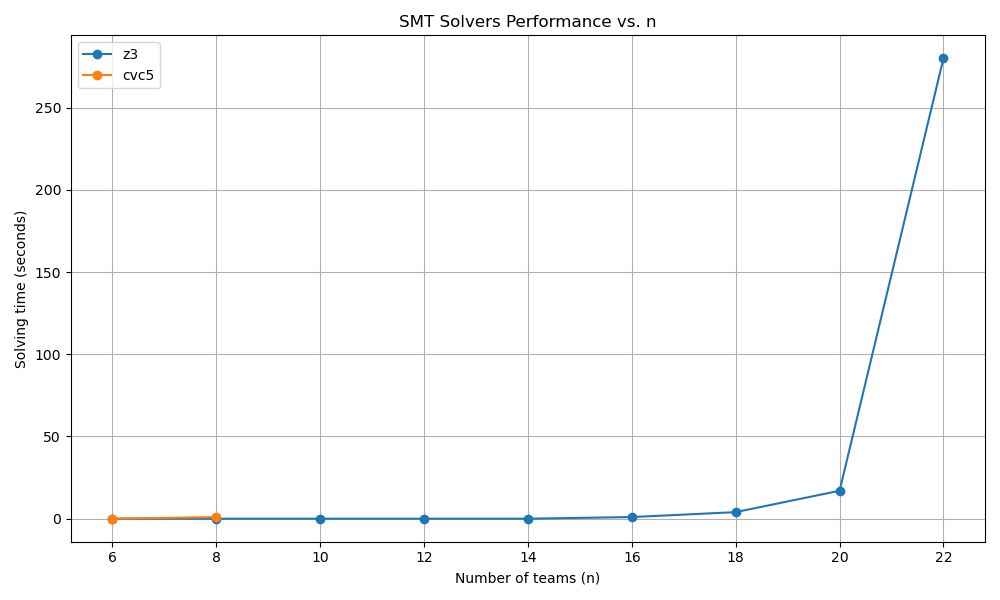
\includegraphics[width=0.8\linewidth]{img/SMT-result.png}
  \caption{SMT solution example}
  \label{fig:smt-result}
\end{figure}

\begin{table}[htbp]
\centering
\small
\begin{tabular}{|c|c|c|}
\toprule
\textbf{n} & \textbf{Z3 (s)} & \textbf{CVC5 (s)} \\
\midrule
6  & 0.11 & 0.13 \\
8  & 0.17 & 1.85 \\
10 & 0.23 & N/A \\
12 & 0.29 & N/A \\
14 & 0.36 & N/A \\
16 & 0.74 & N/A \\
18 & 3.52 & N/A \\
20 & 14.32 & N/A \\
22 & 280.17 & N/A \\
24 & N/A & N/A \\
\bottomrule
\end{tabular}
\caption{SMT solving times}
\label{table:smt-result}
\end{table}
